\chapter{Proprietà termiche dei metalli}
\section{Modello di Drude-Sommerfeld e i suoi problemi}
Il modello di Drude è uno dei primi modelli utilizzati per descrivere i metalli ed è basato sull'ipotesi di un solido perfetto. Le assunzioni di questo modello sono le seguenti:
\begin{itemize}
	\item Gli elettroni vengono trattati come un \textbf{gas ideale di particelle libere}, cioè non interagiscono tra loro né con gli ioni.
	\item Le collisioni tra elettroni sono eventi istantanei e avvengono con una probabilità pari a $\frac{1}{\tau}$, dove $\tau$ è il tempo medio tra collisioni.
	\item Attraverso le collisioni gli elettroni raggiungono l'equilibrio termico.
\end{itemize}
Il fatto che le collisioni siano istantanee e che avvengano con probabilità $\frac{1}{\tau}$ porta ad un meccanismo di attrito interno agli elettroni, il quale comporta una perdita di energia e quindi si manifesta come la resistenza elettrica in un metallo.\\
Tuttavia, \textbf{il modello di Drude risulta adeguato solamente per i metalli alcalini, nei quali gli elettroni si comportano in maniera prossima a particelle libere}, mentre per altri metalli non si ottengono i risultati attesi; ad esempio, il modello fallisce nel prevedere correttamente il calore specifico del metallo.\\\\
Per ovviare a queste problematiche si introduce il \textbf{modello di Drude-Sommerfeld}, che si fonda sui seguenti punti:
\begin{itemize}
	\item Il sistema è formato da \textbf{particelle quantistiche} che interagiscono con gli ioni del reticolo.
	\item Gli elettroni sono considerati quasi-particelle, dotate di una \textbf{massa efficace} diversa dalla massa libera. L'energia dipende dal momento e gli elettroni non interagiscono tra loro.
	\item È necessario utilizzare la \textbf{statistica di Fermi-Dirac}, invece della statistica di Maxwell-Boltzmann, per descrivere la distribuzione delle particelle:
	\[
	f(E)= \frac{1}{e^{\beta (E-\mu)}+1}\,,
	\]
	dove $\beta=\frac{1}{K_B T}$ e $\mu$ è il potenziale chimico.
	\item Si mantiene l'ipotesi che le collisioni siano istantanee e avvengano con una probabilità pari a $\frac{1}{\tau}$.
\end{itemize}
\bigskip
\textbf{Obiettivo:} Ricavare l'energia e la densità degli stati del sistema.

\bigskip
\noindent
Per far ciò consideriamo una scatola cubica di lato $L$ in cui imponiamo le condizioni al contorno di \textbf{Born-Von Karman}, ovvero:
\begin{equation}
	\psi(x,y,z+L)= \psi(x,y,z)\,,
	\label{eqn:condizioni-contorno}
\end{equation}
che descrivono un solido in cui l'elettrone, uscendone da un lato, rientra dall'altro (struttura topologica simile a quella di una ciambella).\\
La soluzione dell'equazione di Schrödinger per elettroni in una scatola con tali condizioni è data da onde piane:
\[
\psi_{\vec{k}}(x,y,z)= \frac{1}{\sqrt{V}} e^{i\vec{k}\cdot\vec{r}}\,,
\]
con energia
\[
\varepsilon(\vec{k})= \frac{\hbar^2 k^2}{2m}\,.
\]
Imponendo la condizione \eqref{eqn:condizioni-contorno} si deduce per la componente $x$, per esempio, che:
\[
e^{i k_x (x+L)}= e^{i k_x x} \quad \implies \quad e^{i k_x L}= 1\,,
\]
da cui
\[
k_x L= 2\pi n_x \quad \Longrightarrow \quad k_x = \frac{2\pi n_x}{L}\,,
\]
con $n_x$ intero. Analogamente si ottengono le quantizzazioni per $k_y$ e $k_z$.\\\\
Calcoliamo la \textbf{densità dei punti $\vec{k}$:} il numero di punti $\vec{k}$ in un volume $\Omega$ dello spazio di $k$ è dato da:
\[
\frac{\Omega}{\left(\frac{2\pi}{L}\right)^3} = \frac{\Omega\, V}{8\pi^3}\,,
\]
da cui la densità dei punti, cioè il numero di stati per unità di volume di $k$, è:
\begin{equation}
	\rho = \frac{V}{8\pi^3}\,.
	\label{eqn:densita_k}
\end{equation}

\bigskip
\noindent
In un solido ci sono circa $10^{22}$ elettroni che si distribuiscono nei vari stati disponibili, riempiendo il livello fondamentale e successivamente tutti gli stati fino al livello di Fermi, generando la cosiddetta \textbf{sfera di Fermi} di raggio $k_f$. \\
Il numero di elettroni contenuti nella sfera di Fermi è dato da:
\[
\underbrace{\left(\frac{4\pi k_f^3}{3}\right)}_{\text{Volume della sfera}} \cdot \frac{V}{8\pi^3}\,.
\]
Ricordando che ad ogni stato sono associati due elettroni (degenerazione di spin), si ha:
\begin{equation}
	N= 2\cdot \frac{V}{8\pi^3} \cdot \frac{4\pi k_f^3}{3} = \frac{V}{3\pi^2} k_f^3\,.
	\label{eqn:N_V}
\end{equation}
La densità elettronica (numero di elettroni per unità di volume) è quindi:
\[
n= \frac{N}{V}= \frac{k_f^3}{3\pi^2}\,.
\]

\bigskip
\noindent
L'energia di Fermi è:
\begin{equation}
	E_f= \frac{\hbar^2 k_f^2}{2m}\,.
	\label{eqn:Ef}
\end{equation}

\bigskip
\noindent
Un'altra quantità utile è il volume per elettrone, $v= \frac{V}{N}$, da cui si può definire una lunghezza caratteristica $\sqrt[3]{v}\equiv n_0$. Inoltre, per un metallo generico si può esprimere il vettore di Fermi nel seguente modo (in unità appropriate):
\[
k_f = \frac{3.63}{r\, a_0} \, \text{\AA}^{-1} \quad \text{oppure} \quad v_f= \left(\frac{\hbar}{m}\right) k_f \approx 0.01 \cdot c\,,
\]
dove $c$ è la velocità della luce, e l'energia di Fermi assume valori tipici tra \SI{1.5} e \SI{15}{\electronvolt}, corrispondenti a temperature di Fermi dell'ordine:
\[
T_f= \frac{E_f}{K_B} \approx \frac{58.2}{(r/a_0)^2} \times 10^4\, \text{K}\,.
\]
Quindi, a temperatura ambiente, gli elettroni occupano lo stato fondamentale.

\bigskip
\noindent
\textbf{Calcolo dell'energia media degli elettroni:}\\
L'energia totale del sistema si esprime come:
\[
E= 2\sum_{0< k< k_f} \frac{\hbar^2 k^2}{2m}\,,
\]
dove il fattore 2 deriva dalla degenerazione di spin. Convertendo la somma in integrale, si introduce la densità dei punti $\vec{k}$ (\ref{eqn:densita_k}). Quindi:
\[
\frac{E}{V}= 2 \int \frac{d\vec{k}}{8\pi^3} \frac{\hbar^2 k^2}{2m}\,.
\]
Utilizzando le coordinate sferiche, l'integrale diventa:
\[
\frac{E}{V}= 2 \cdot \frac{1}{8\pi^3} \cdot 4\pi \int_0^{k_f} \frac{\hbar^2}{2m} k^4 \, dk = \frac{\hbar^2}{2m} \cdot \frac{1}{\pi^2} \int_0^{k_f} k^4\, dk\,.
\]
Eseguendo l'integrale:
\[
\int_0^{k_f} k^4\, dk= \frac{k_f^5}{5}\,,
\]
si ottiene:
\[
\frac{E}{V}= \frac{1}{\pi^2} \cdot \frac{\hbar^2 k_f^5}{10m}\,.
\]
Pertanto, l'energia media per particella è:
\[
\frac{E}{N}= \frac{E}{V}\cdot \frac{V}{N}= \frac{1}{\pi^2} \cdot \frac{\hbar^2 k_f^5}{10m} \cdot \frac{3\pi^2}{k_f^3} = \frac{3}{5} \varepsilon_f\,,
\]
dato che, da (\ref{eqn:Ef}), $\varepsilon_f=\frac{\hbar^2 k_f^2}{2m}$. Di conseguenza l'energia totale risulta:
\[
E= \frac{3}{5}\varepsilon_f N\,.
\]
Si osserva che questa energia per particella è relativamente elevata.

\bigskip
\section{Proprietà termiche e calore specifico nei metalli}

La relazione tra l'energia di Fermi e il potenziale chimico $\mu$ è data dalla condizione a $T=0$:
\[
\mu(T=0)= \varepsilon_f\,.
\]
A temperature maggiori di zero, $\mu$ si sposta rispetto a $\varepsilon_f$, come mostrato in figura (vedi Figura \ref{fig:FDTmagg0}). 
\begin{figure} [H]
	\centering
	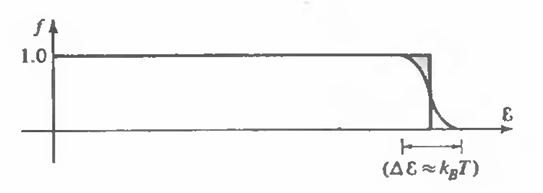
\includegraphics[width=0.6\textwidth]{images/1-Proprietà-Metalli/FDTmagg0.png}
	\caption{all'aumentare della temperatura la distribuzione di Fermi Dirac non è più una funzione a gradino}
	\label{fig:FDTmagg0}
\end{figure}

In tale grafico si nota che, all'aumentare della temperatura, la distribuzione di Fermi-Dirac non mantiene più la forma a gradino, ma si arrotonda. Le particelle che vengono "spostate" a destra (oltre il livello di Fermi) sono quelle che contribuiscono alla conduzione.\\\\
Per stimare le variazioni energetiche a temperatura finita si osserva che le particelle che cambiano stato sono quelle in un intorno di ampiezza $\sim K_B T$ intorno a $\varepsilon_f$. Se il numero di queste particelle è pari a $g(E_f) \cdot K_B T$, e ciascuna acquisisce in media un'energia dell'ordine di $K_B T$, allora la variazione di energia è:
\[
\Delta U \approx g(E_f) (K_B T)^2\,.
\]
Pertanto il calore specifico (per unità di volume) è:
\begin{equation}
	\frac{\partial \Delta U}{\partial T} \approx 2 K_B^2 T\,g(E_f)\,.
	\label{eqn:Cv_explicit}
\end{equation}
Questa correzione al calore specifico spiega il comportamento sperimentale, in cui il calore specifico diminuisce tendendo a zero quando $T\to 0$, contrariamente al caso classico in cui si avrebbe un calore specifico costante $C_V = 3R$.

\bigskip
\noindent
Analizziamo ora la dipendenza dell'energia totale $U$ (o della densità energetica $u=\frac{U}{V}$) dalla temperatura. L'energia totale del sistema è data da:
\[
U= 2 \sum_{\vec{k}} \varepsilon(\vec{k})\, f(\varepsilon(\vec{k}))\,,
\]
dove $f(\varepsilon)$ è la distribuzione di Fermi-Dirac. Passando dalla somma ad un integrale, si ha:
\[
u= \frac{U}{V}= 2\int \frac{d\vec{k}}{8\pi^3} \varepsilon(\vec{k})\, f(\varepsilon(\vec{k}))\,.
\]
Utilizzando la relazione tra lo spazio dei vettori $k$ ed il numero di stati in funzione dell'energia, si introduce la densità degli stati $g(\varepsilon)$; pertanto:
\[
u= \int_{0}^{\infty} d\varepsilon\, g(\varepsilon)\, \varepsilon\, f(\varepsilon)\,,
\]
e analogamente la densità delle particelle è:
\[
n= \int_{0}^{\infty} d\varepsilon\, g(\varepsilon)\, f(\varepsilon)\,.
\]

A temperature finite, per calcolare integrali del tipo 
\[
I= \int_{-\infty}^{\infty} H(\varepsilon) f(\varepsilon)\,d\varepsilon\,,
\]
è utile espandere $H(\varepsilon)$ in un intorno del potenziale chimico $\mu$. L'espansione (nota come espansione di Sommerfeld) è:
\[
\int_{-\infty}^{\infty} H(\varepsilon) f(\varepsilon) d\varepsilon = \int_{-\infty}^{\mu} H(\varepsilon) d\varepsilon + \frac{\pi^2}{6}(K_B T)^2\, H'(\mu) + O\left(\frac{K_B T}{\mu}\right)^4\,.
\]
Applicando questa espansione sia per $u$ che per $n$, e limitando l'integrazione da 0 a $\mu$ (poiché $g(\varepsilon)=0$ per $\varepsilon<0$), si ottengono:
\[
u= \int_0^\mu \varepsilon\, g(\varepsilon)\,d\varepsilon + \frac{\pi^2}{6}(K_B T)^2 \left[\varepsilon\,g'(\mu)+ g(\mu)\right] + O(T^4)
\]
e
\[
n= \int_0^\mu g(\varepsilon)\,d\varepsilon + \frac{\pi^2}{6}(K_B T)^2\, g'(\mu) + O(T^4)\,.
\]
Il potenziale chimico cambia con la temperatura e non coincide perfettamente con l'energia di Fermi, per cui si attua una seconda espansione:
\[ \int_0^\mu H(\varepsilon) d\varepsilon = \int_0^{\varepsilon_f} H(\varepsilon)d(\varepsilon) + (\mu - \varepsilon_f) H(\varepsilon_f) \]
Quindi ottengo:
\[ u = \int_0^{\varepsilon_f} \varepsilon\cdot  g(\varepsilon)\dot d\varepsilon  + (\mu - \varepsilon_f) g(\varepsilon_f)\cdot \varepsilon_f  + \frac{\pi^2}{6}(K_b T)^2 \bigl[g'(\varepsilon_f)  + g(\varepsilon_f)\bigr]+ O(T^4) \]
\[ n = \int_0^{\varepsilon_f} g(\varepsilon)\cdot d\varepsilon +\left\{(\mu - \varepsilon_f) g(\varepsilon_f) + \frac{\pi^2}{6}(K_b T)^2 g'(\varepsilon_f) \right\} \]
siccome $\int_0^\mu g(\varepsilon)d\varepsilon = n$ per definizione, questo significa che  \\
\[\left\{(\mu - \varepsilon_f) g(\varepsilon_f) + \frac{\pi^2}{6}(K_b T)^2 g'(\varepsilon_f) \right\} = 0\]
altrimenti non sto conservano il numero totale di particelle nel caso degli elettroni, da questa relazione possiamo quindi ricavare il poetnziale chimico:
\begin{equation}
	\mu = \varepsilon_f - \frac{\pi^2}{6} (K_b T)^2 \cdot \frac{g'(\varepsilon_f) }{g(\varepsilon_f) }
	\label{eqn:muT}
\end{equation}
Il segno del termine correttivo dipende dal segno di $g'(\varepsilon_f)$ e ciò spiega il piccolo spostamento di $\mu$ con la temperatura, come illustrato ad esempio in Figura \ref{fig:fermidirac2}.
\begin{figure} [H]
	\centering
	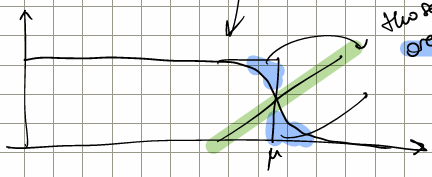
\includegraphics[width=0.4\textwidth]{images/1-Proprietà-Metalli/fermidirac2.png}
	\caption{}
	\label{fig:fermidirac2}
\end{figure}

\bigskip
\subsection{Densità di stati}

Quanti stati hanno energia compresa tra $\varepsilon$ e $\varepsilon + d\varepsilon$? In generale la densità di stati è definita da:
\begin{equation}
	g(\varepsilon)= \int \frac{d\vec{k}}{4\pi^3} \, \delta(\varepsilon-\varepsilon(\vec{k}))\,.
	\label{eqn:dos_def}
\end{equation}
Per valutare questo integrale, anziché lavorare direttamente con la delta di Dirac, si conta il numero di stati in una corona sferica nel $k$-space. La relazione tra una variazione infinitesima di energia $d\varepsilon$ e quella di $k$ è data da:
\[
\varepsilon + d\varepsilon \approx \varepsilon + |\vec{\nabla} \varepsilon(k)|\, \delta k(k) \quad \Longrightarrow \quad \delta k(k)= \frac{d\varepsilon}{|\vec{\nabla} \varepsilon(k)|}\,.
\]
\begin{figure} [H]
	\centering
	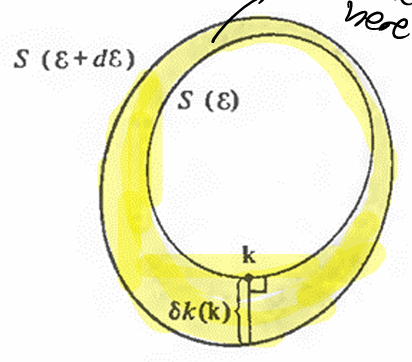
\includegraphics[width=0.4\textwidth]{images/1-Proprietà-Metalli/coronacircolare.png}
	\caption{}
	\label{fig:corona-circolare}
\end{figure}

Pertanto, il numero di stati con energia compresa in $[\varepsilon,\varepsilon+d\varepsilon]$ è:
\[
g(\varepsilon) \, d\varepsilon = \int_{S(\varepsilon)} \frac{dS}{4\pi^3}\,\frac{d\varepsilon}{|\vec{\nabla} \varepsilon(k)|}\,,
\]
da cui
\[
g(\varepsilon)= \int_{S(\varepsilon)} \frac{dS}{4\pi^3}\,\frac{1}{|\vec{\nabla} \varepsilon(k)|}\,.
\]
 In 3D $g(\varepsilon)$ è integrabile ma ci sono delle divergenze di $\frac{dg}{d\varepsilon}$ chiamate \textbf{singolarità di van Hove}, e sono mostrate in Figura \ref{fig:densstati3D}\\\\
\begin{figure} [H]
	\centering
	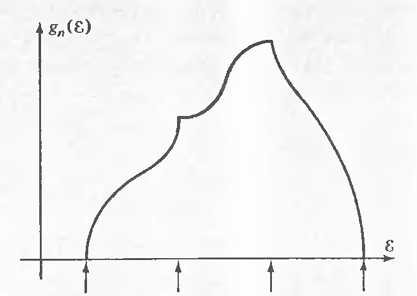
\includegraphics[width=0.4\textwidth]{images/1-Proprietà-Metalli/densstati3d.png}
	\caption{in figura i punti critici vengono indicati dalle frecce}
	\label{fig:densstati3D}
\end{figure}

Nel caso in cui
\[
\varepsilon(k)= \frac{\hbar^2 k^2}{2m}\,,
\]
si ha, in 1D, la derivata:
\[
\frac{d\varepsilon}{dk}= \frac{\hbar^2 k}{m}\,,
\]
e passando all'integrazione in $k$-space in 3D, contando il numero di stati in una corona sferica (tenendo conto della degenerazione di spin), il numero di stati tra $k$ e $k+dk$ è dato da:
\[
g(\varepsilon)d\varepsilon= 2\cdot \frac{1}{8\pi^3}\cdot 4\pi k^2\, dk\,.
\]
Poiché
\[
\frac{d\varepsilon}{dk}= \frac{\hbar^2 k}{m} \quad \Longrightarrow \quad dk= \frac{m}{\hbar^2 k}\,d\varepsilon\,,
\]
si ottiene:
\[
g(\varepsilon)= \frac{1}{\pi^2}\, k^2 \cdot \frac{m}{\hbar^2 k}= \frac{m}{\pi^2 \hbar^2}\, k\,.
\]
Infine, esprimendo $k$ in funzione dell'energia:
\[
k= \sqrt{\frac{2m\varepsilon}{\hbar^2}}\quad \implies \quad g(\varepsilon)= \frac{m}{\pi^2 \hbar^2}\sqrt{\frac{2m\varepsilon}{\hbar^2}} \propto \sqrt{\varepsilon}\,.
\]
Questo risultato corrisponde al noto andamento di $g(\varepsilon)$ nei metalli. In figura (vedi Figura \ref{fig:dosvsen}) si mostra l'andamento della densità degli stati moltiplicata per la distribuzione di Fermi-Dirac.
\begin{figure} [H]
	\centering
	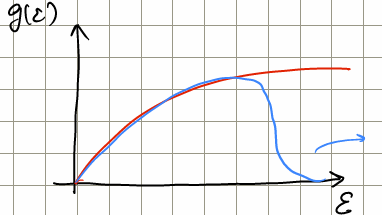
\includegraphics[width=0.4\textwidth]{images/1-Proprietà-Metalli/dosvsen.png}
	\caption{l'occupazione degli stati è indicata dalla curva in azzurro ed è così perchè è moltiplicata per la distribuzione di Fermi dirac}
	\label{fig:dosvsen}
\end{figure}

\subsection{Calcolo dell'energia totale e del calore specifico}
La densità di energia totale invece è data da:
\begin{equation}
\begin{split}
     u &= \int_0^{\varepsilon_f} \varepsilon\cdot  g(\varepsilon)\dot d\varepsilon  + \cancel{(\mu - \varepsilon_f) g(\varepsilon_f)\cdot \varepsilon_f}  + \cancel{\frac{\pi^2}{6}(K_b T)^2 \bigl[g'(\varepsilon_f)}  + g(\varepsilon_f)\bigr] \\
     &= \int_0^{\varepsilon_f} \varepsilon \ g(\varepsilon_f) d\varepsilon + \frac{\pi^2}{6} (KT)^2g(\varepsilon_f) = u_0 +  \frac{\pi^2}{6} (KT)^2g(\varepsilon_f)
\end{split}
\end{equation}
dove $\int_0^{\varepsilon_f} \varepsilon \ g(\varepsilon_f) d\varepsilon = u_0(T=0)$. \\\\
Da cui ottengo:
\begin{equation}
    C_v =\frac{du}{dt}\biggr|_v =\frac{\pi^2}{3}\cdot K_b^2T\cdot g(\varepsilon_f)
    \label{eqn:uconu0}
\end{equation}
Questo risultato, in accordo con le misurazioni sperimentali, mostra che il contributo degli elettroni al calore specifico è proporzionale a $T$ per $T\to 0$, mentre il contributo classico (basato sui soli gradi di libertà armonici) darebbe un valore costante.

\bigskip
\noindent
Si nota infine che, in un metallo, solo una piccola frazione degli elettroni (quelli prossimi a $\varepsilon_f$, il cosiddetto "strato di superficie" della sfera di Fermi, dell'ordine di $\sim K_B T$) è in grado di partecipare al trasporto termico e alla conduzione elettrica; il resto degli elettroni resta vincolato negli stati profondi e non contribuisce alle proprietà termiche a basse temperature.

\bigskip
\subsection{Calcolo esplicito della densità degli stati all'energia di Fermi}
Calcoliamo la densità di stati all'energia di Fermi. L'energia di Fermi in funzione di n è data da: $\varepsilon_f = \frac{\hbar^2}{2m}(3\pi^2 n)^{\frac{2}{3}}$ quindi:
\[ g(\varepsilon_f) = \frac{m}{\hbar^2 \pi^2} \sqrt{\frac{2m}{\hbar^2}} \sqrt{\varepsilon_f} \]
moltiplico e divido per $\frac{3}{2}\cdot n$ e ottengo:
\[ g(\varepsilon_f) =  \frac{3n}{2} \frac{2}{3n} \frac{m}{\hbar^2 \pi^2} \sqrt{\frac{2m}{\hbar^2}} \sqrt{\varepsilon_f} =  \frac{3n}{2} \left[ \left( \frac{1}{3\pi^2 n} \right) \left( \frac{2m}{\hbar^2} \right)^{\frac{3}{2}} \sqrt{\varepsilon_f} \right] = \frac{3n}{2} \frac{{\varepsilon_f}^\frac{1}{2}}{\varepsilon_f^{\frac{3}{2}}} = \frac{3}{2} \frac{n}{\varepsilon_f} \]
\[ \implies \mu =  \varepsilon_f - \frac{\pi^2}{6} (K_b T)^2 \frac{g'(\varepsilon_f) }{g(\varepsilon_f) }= [g(\varepsilon) \propto \sqrt{\varepsilon}] = \varepsilon_f \left[ 1 - \frac{1}{3} \left( \frac{\pi K_b T}{2 \varepsilon_f} \right)^2 \right] \]
considerando il calore specifico nella \ref{eqn:uconu0} nel caso dei metalli alcalini si ottiene:
\[ C_v = \left( \frac{\partial u}{\partial T} \right)_n = \frac{\pi^2}{3} K_b^2 T \ g(\varepsilon_f) = \frac{\pi^2}{2}\frac{n}{\varepsilon_f}K_b^2\cdot T\]
Confrontando con il risultato classico, che darebbe (utilizzando il modello di Einstein per i fononi, ad esempio):
\[
u= \frac{9}{2}\, K_B\, T\, n \quad \Longrightarrow \quad C_v^{\text{classico}}= \frac{9}{2}\,K_B\, n\,,
\]
si evidenzia come, a temperatura ambiente, solo una piccolissima frazione degli elettroni (quelli in prossimità di $\varepsilon_f$) contribuisce al calore specifico, mentre la maggior parte degli elettroni (al di sotto dell'energia di Fermi) rimane "congelata" e non partecipa all'aumento di energia termica.

\bigskip
\noindent
In Figura \ref{fig:cvCLvsQ} viene mostrato un confronto tra il calore specifico classico (costante, in nero) e quello corretto (che cresce linearmente con $T$, in viola), in cui la linea tratteggiata indica la temperatura ambiente.

\begin{figure}[H]
	\centering
	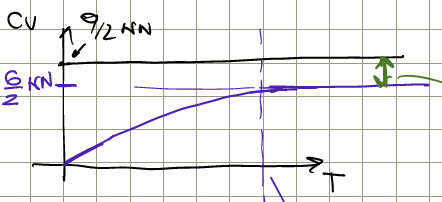
\includegraphics[width=0.5\textwidth]{images/1-Proprietà-Metalli/cvCLvsQ.png}
	\caption{Confronto tra il comportamento classico (costante) del calore specifico e il comportamento corretto (lineare in $T$) per i metalli.}
	\label{fig:cvCLvsQ}
\end{figure}

\bigskip
\noindent
Infine, si osserva che il numero di elettroni che "saltano" (cioè, che modificano il loro stato energetico a causa dell'aumento termico) è estremamente piccolo rispetto al numero totale, come illustrato in Figura \ref{fig:FD3}.

\begin{figure}[H]
	\centering
	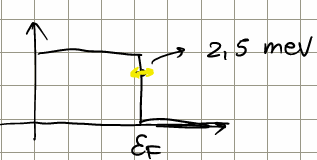
\includegraphics[width=0.5\textwidth]{images/1-Proprietà-Metalli/FD3.png}
	\caption{Distribuzione di Fermi-Dirac che evidenzia la piccola frazione di elettroni attivi (vicino a $\varepsilon_f$) a temperatura ambiente.}
	\label{fig:FD3}
\end{figure}